\documentclass[12pt]{article}
\usepackage{enumitem}
\usepackage{setspace}
\usepackage{graphicx}
\usepackage{subcaption}
\usepackage{amsmath, amsthm}
\usepackage{booktabs}
\RequirePackage[colorlinks]{hyperref}
\usepackage[lined,boxed,linesnumbered,commentsnumbered]{algorithm2e}
\usepackage{xcolor}
\usepackage{listings}
\lstset{basicstyle=\ttfamily,
  showstringspaces=false,
  commentstyle=\color{red},
  keywordstyle=\color{blue}
}

% Margins
\topmargin=-0.45in
\evensidemargin=0in
\oddsidemargin=0in
\textwidth=6.5in
\textheight=9.0in
\headsep=0.25in

\linespread{1.1}

% Commands
\newenvironment{solution}
  {\begin{proof}[Solution]}
  {\end{proof}}

\title{CSE6250: Big Data Analytics in Healthcare \\ Homework 5}
\author{Richard Albright (GTID: 903548616)}
\date{\today}

\begin{document}

\maketitle

\section{Epileptic Seizure Classification}

\subsection*{1.2 Multi-layer Perceptron}
~

\textbf{b.} Calculate the number of "trainable" parameters in the model with providing the calculation details. How many floating-point computation will occur when a new single data point comes in to the model?  \textbf{You can make your own assumptions on the number of computations made by each elementary arithmetic, e.g., add/subtraction/multiplication/division/negation/exponent take 1 operation, etc.} [5 points]

\bigskip

\textbf{MLP Original Model - Trainable Parameters}

Input Layer - 178 Input Features, 16 Output Features

Hidden Layer Weights: 178 * 16 = 2848 + 16 Bias Terms = 2864

Output Layer = 16 Input Features, 5 Output Features

Output Layer Weights: 80 + 5 Bias Terms = 85

\textbf{Total Trainable Parameters = 2949}

\bigskip

\textbf{MLP Improved Model - Trainable Parameters}

Input Layers - 178 Input Features, 89 Output Features

1st Hidden Layer Weights: 178*89 = 15842, + 89 Bias Terms = 15931

2nd Hidden Layer - 89 Input Features, 44 Output Features

2nd Hidden Layer Weights = 89 * 44 = 3916, + 44 Bias Terms = 3960

3rd Hidden Layer - 44 Input Featuresm 22 Output Features

3rd Hidden layer Weights: 44 * 22 = 968, + 22 Bias Terms = 990

4th Hidden Layer - 22 Input Features, 10 Output Features

4th Hidden Layer Weights = 22 * 10 = 220, + 10 Bias Terms = 230

Output Layer, 10 Input Features, 5 Output Features

Output Layer Weights = 10 * 5 = 50 + 5 Bias Terms = 55

\textbf{Total Trainable Parameters = 21116}

\bigskip

\textbf{MLP Original Model - Operations Count}

178 * 16 * 16 = 45568

16 * 5 * 5 = 400

968 * 22 = 21296

220 * 10 = 2200

50 * 5  = 250

= 69706

\bigskip

\textbf{MLP Improved Model - Operations Count}

178 * 89 * 89 = 1409938

89 * 44 * 44 = 172304

968 * 22 = 21296

220 * 10 = 2200

50 * 5  = 250

= 1605988



\bigskip

\textbf{c.} Attach the learning curves for your MLP model in your report. [2 points]

\bigskip

Original Model Left, Improved Model Right

\bigskip

{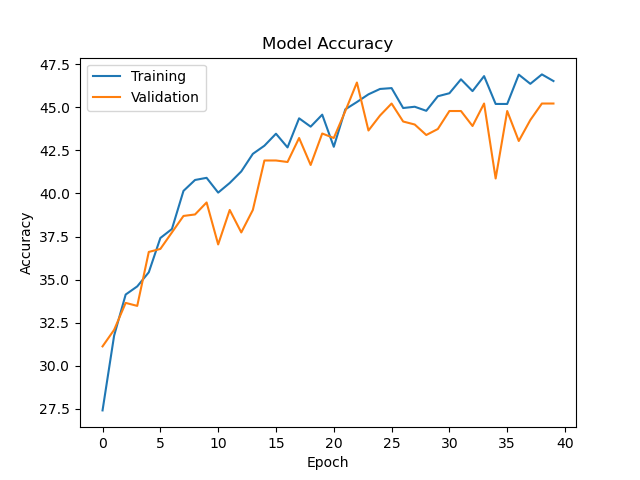
\includegraphics[width = 3in]{images/MLP_accuracies}
{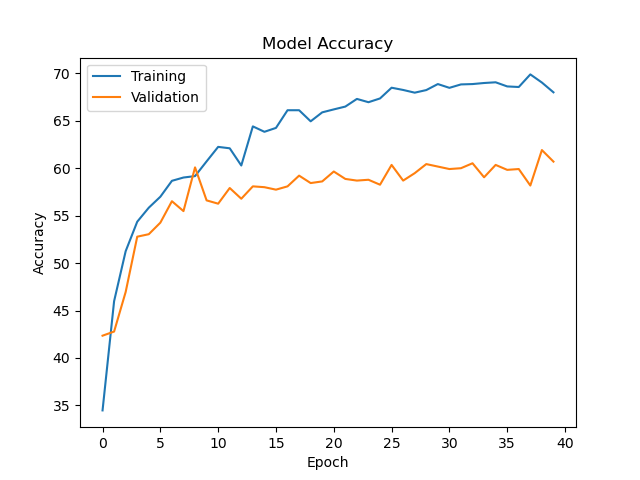
\includegraphics[width = 3in]{images/MLP_improved_accuracies}

\bigskip

Original Model Left, Improved Model Right

\bigskip

{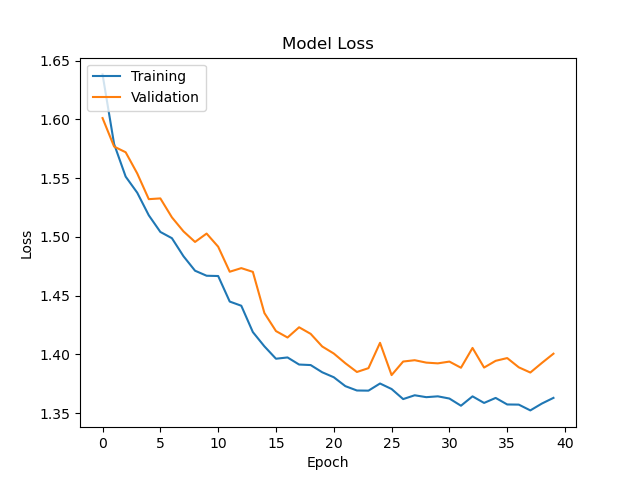
\includegraphics[width = 3in]{images/MLP_losses}
{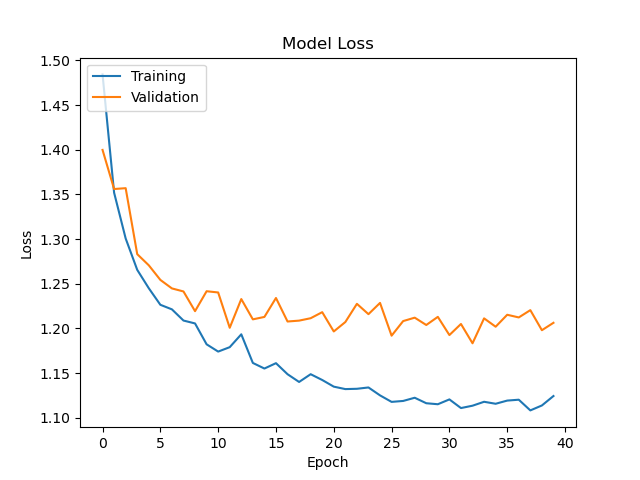
\includegraphics[width = 3in]{images/MLP_improved_losses}


\textbf{d.} Attach the confusion matrix for your MLP model in your report. [2 points]

\bigskip

Original Model Left, Improved Model Right

\bigskip

{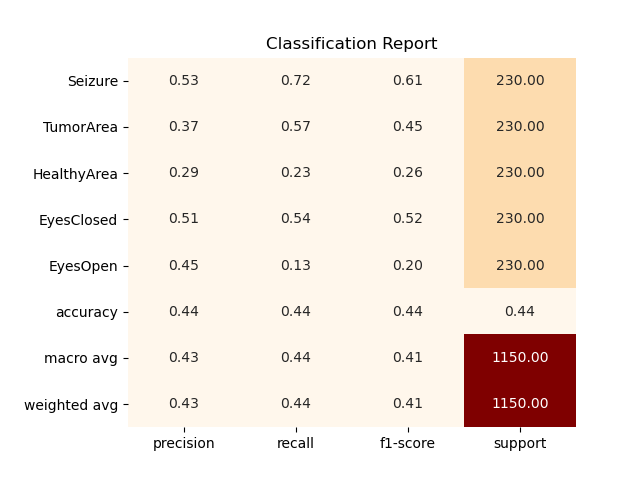
\includegraphics[width = 3in]{images/MLP_classification_report}
{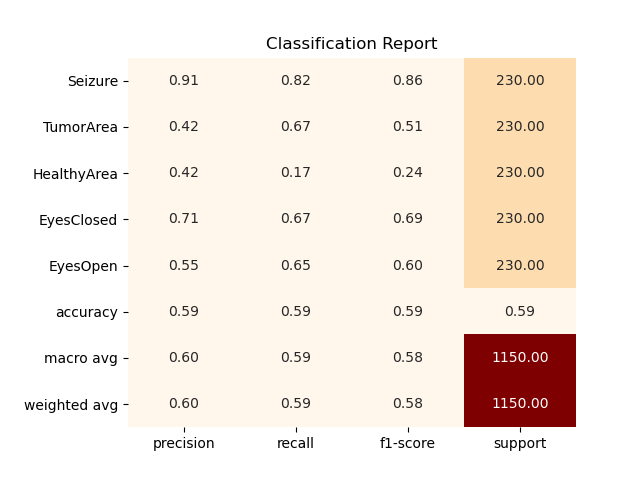
\includegraphics[width = 3in]{images/MLP_improved_classification_report}

\bigskip

Original Model Left, Improved Model Right

\bigskip

{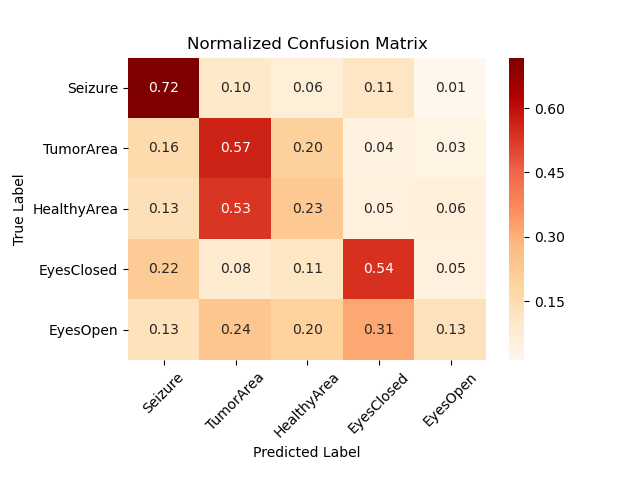
\includegraphics[width = 3in]{images/MLP_confusion_matrix}
{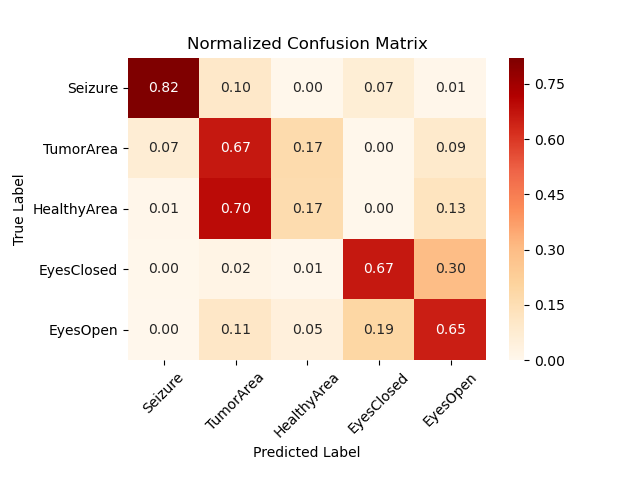
\includegraphics[width = 3in]{images/MLP_improved_confusion_matrix}

\bigskip

\textbf{e.} Explain your architecture and techniques used. Briefly discuss about the result with plots. [3 points]

\bigskip

My MLP model consisted of a 6 layer model, it consisted of 4 hidden layers and an ouput layer that are fully connected, followed by a sigmoid activation function.  The 1st layer has 178 inputs and 89 outputs.  The 2nd layer has 89 inputs and 44 outputs.  The 3rd layer has 44 inoputs and 22 outputs.  The 4th layer has 22 inputs and 10 outputs, The output layer has 10 inputs and 5 outputs, The sidmoid activation function is called on the output layer. 

\bigskip

Overall Accuracy of the improved model increased 0.15, from 0.44 to 0.59. There were improvements in all clasifications except for the Healthy Area Label, which dropped from an accuracy rate of 0.23 to 0.17.  All other classifications accuracies increased by at least 0.10.  The improved model is a bit overtrained a the validation line is a bit lower than the training line on the accuracy plots and a bit higher than triaing line on the loss plots.


\subsection*{1.3 Convolutional Neural Network (CNN)}
~

\textbf{b.} Calculate the number of "trainable" parameters in the model with providing the calculation details. How many floating-point computation will occur when a new single data point comes in to the model?  \textbf{You can make your own assumptions on the number of computations made by each elementary arithmetic, e.g., add/subtraction/multiplication/division/negation/exponent take 1 operation, etc.} [5 points]

\bigskip

\textbf{CNN Original Model - Trainable Parameters}

1st Convolutional Layer - 1 Input Channel, 6 Output Channels, Kernel Size 5, Stride 1

1st Convolutional Layer Weights: 5 * 6 = 30, + 6 Bias Terms = 36

Pooling Layer - Kernel Size 2, Stride 2, Dilation 1, Padding 0

2nd Convolutional Layer - 6 Input Channels, 16 Ouput Channels, Kernel Size 5, Stride 1

2nd Convolutional Layer Weights: 16 * 5 * 6 = 480, + 16 Bias Terms = 496

Pooling Layer - Kernel Size 2, Stride 2, Dilation 1, Padding 0

1st Linear Layer - Input Features = 16 * 41 = 656, Output Features = 128

1st Linear Layer Weights: 656 * 128 = 83968, + 128 Bias Terms = 84096

2nd Linear Layer - 128 Input Features, 5 Output Features

2nd Linear Layer Weights: 128 * 5 = 640, + 5 Bias Terms = 645

\textbf{Total Trainable Parameters = 85273}
  
\bigskip

\textbf{CNN Improved Model - Trainable Parameters}

1st Convolutional Layer - 1 Input Channel, 6 Output Channels, Kernel Size 5, Stride 1

1st Convolutional Layer Weights: 5 * 6 = 30, + 6 Bias Terms = 36

Pooling Layer - Kernel Size 2, Stride 2, Dilation 1, Padding 0

2nd Convolutional Layer - 6 Input Channels, 16 Ouput Channels, Kernel Size 5, Stride 1

2nd Convolutional Layer Weights: 16 * 5 * 6 = 480, + 16 Bias Terms = 496

Pooling Layer - Kernel Size 2, Stride 2, Dilation 1, Padding 0

1st Linear Layer - Input Features = 16 * 41 = 656, Output Features = 512

1st Linear Layer Weights: 656 * 512 = 335872, + 512 Bias Terms = 336384

2nd Linear Layer - 512 Input Features, 256 Output Features

2nd Linear Layer Weights: 512 * 256 = 131072, + 256 Bias Terms = 131328

3rd Linear Layer - 256 Input Features, 128 Output Features

3rd Linear Layer Weights: 256 * 128 = 32768, + 128 Bias Terms = 32796

4th Linear Layer - 128 Input Features, 64 Output Features

4th Linear Layer Weights: 128 * 64 = 8192, + 64 Bias Terms = 8256

Output Layer - 64 Input Features, 5 Output Features

Output Layer Weights: 64 * 5 = 320, + 5 Bias Terms = 325

\textbf{Total Trainable Parameters = 509721}

\bigskip

\textbf{CNN Original Model - Operation Count}

\bigskip

\textbf{CNN Improved Model - Operation Count}

\bigskip

\textbf{c.} Plot and attach the learning curves and the confusion matrix for your CNN model in your report. [2 points]

\bigskip

Original Model Left, Improved Model Right

\bigskip

{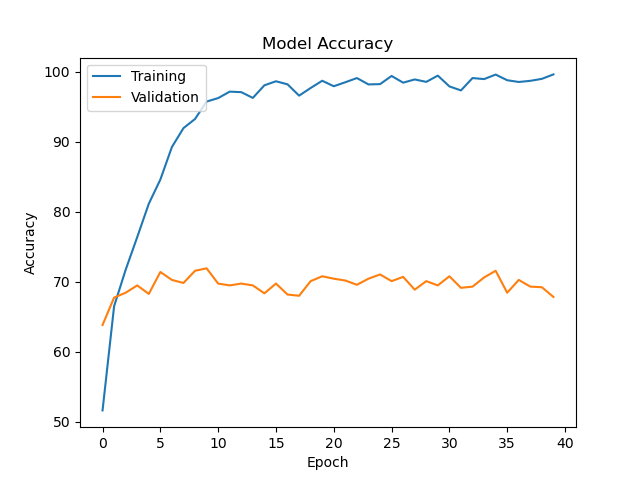
\includegraphics[width = 3in]{images/CNN_accuracies}
{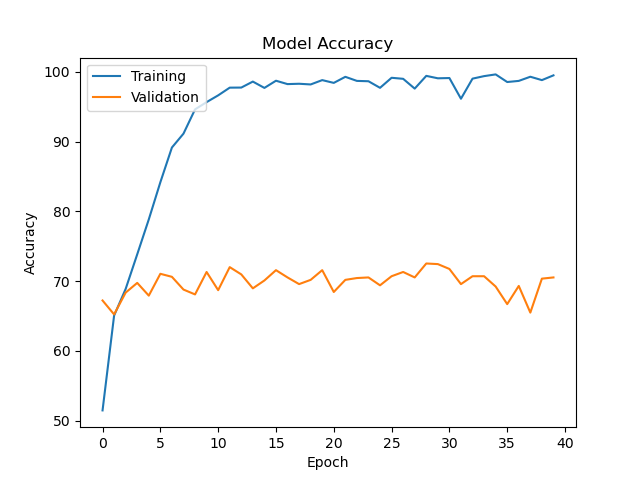
\includegraphics[width = 3in]{images/CNN_improved_accuracies}

\bigskip

Original Model Left, Improved Model Right

\bigskip

{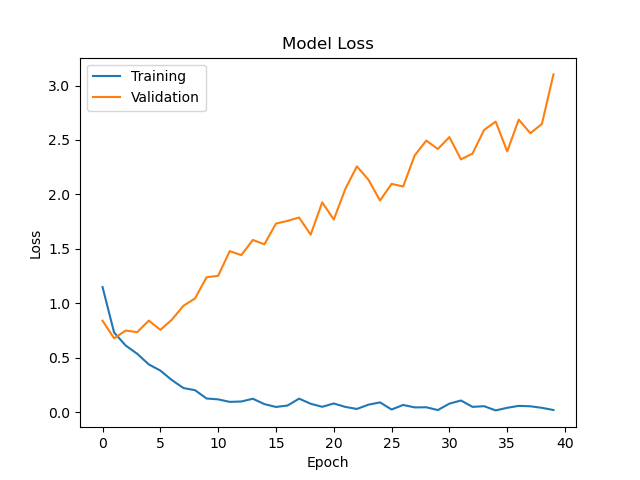
\includegraphics[width = 3in]{images/CNN_losses}
{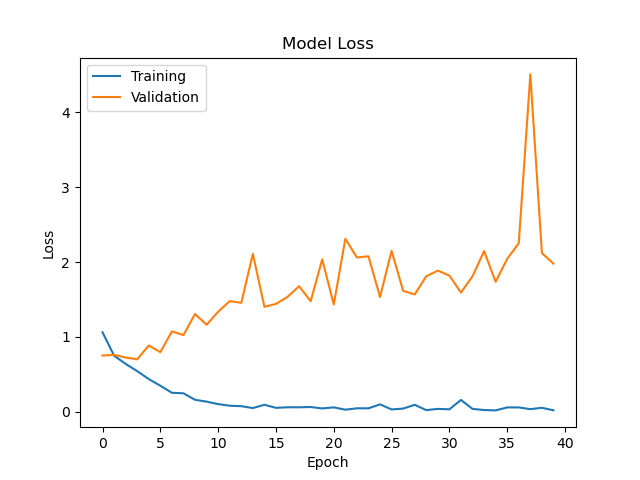
\includegraphics[width = 3in]{images/CNN_improved_losses}

\bigskip

Original Model Left, Improved Model Right

\bigskip

{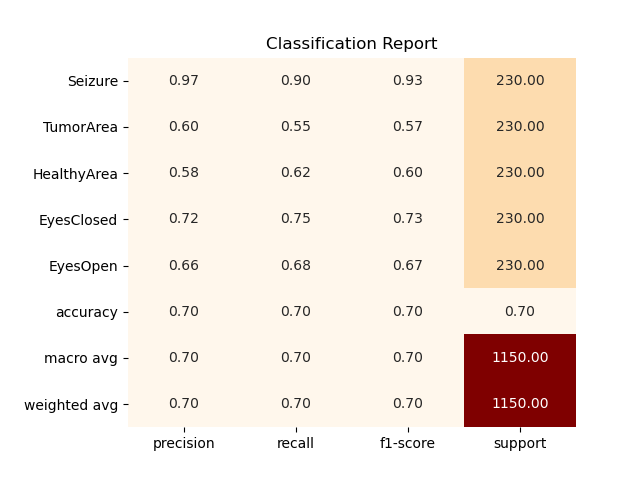
\includegraphics[width = 3in]{images/CNN_classification_report}
{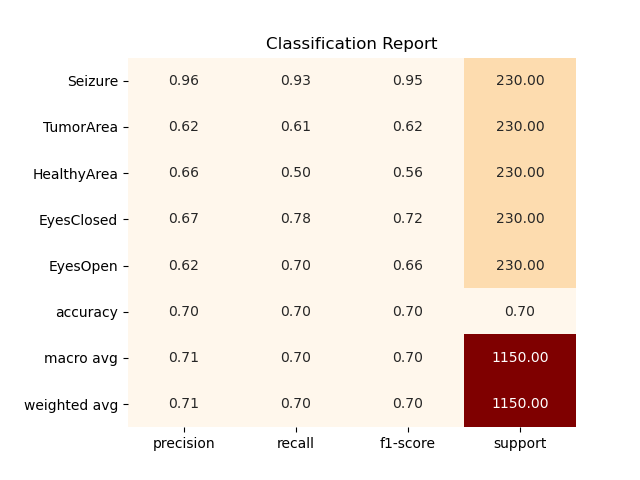
\includegraphics[width = 3in]{images/CNN_improved_classification_report}

\bigskip

Original Model Left, Improved Model Right

\bigskip

{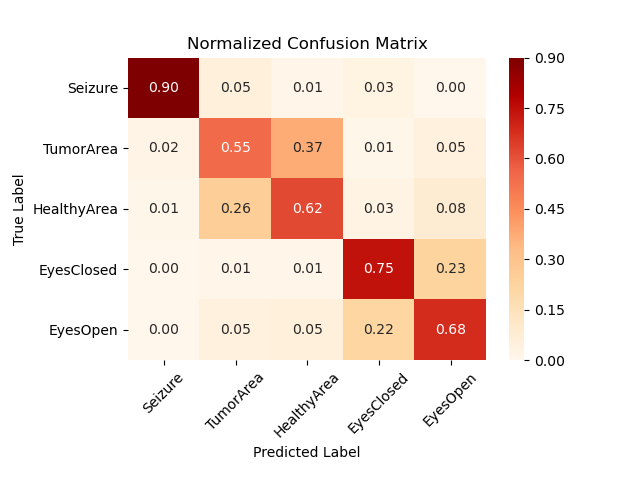
\includegraphics[width = 3in]{images/CNN_confusion_matrix}
{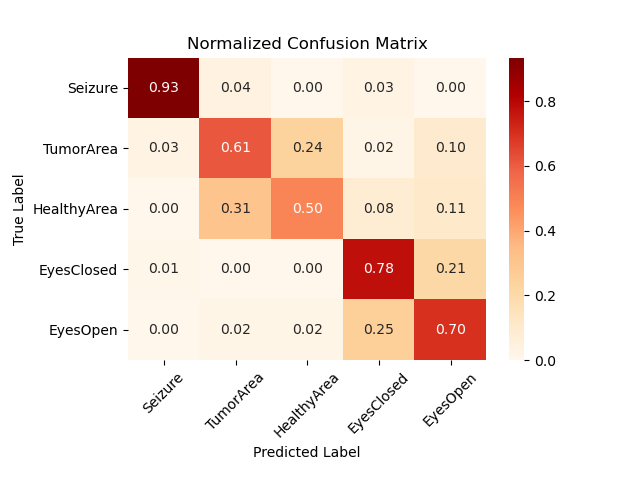
\includegraphics[width = 3in]{images/CNN_improved_confusion_matrix}

\bigskip
\textbf{d.} Explain your architecture and techniques used. Briefly discuss about the result with plots. [3 points]

\bigskip

My CNN improved model makes use of adding fully connected layers after the convolutional layers.  The original model has 128 features output from the convolutional layers, while the improved model outputs 512 features.  The subsequent layers are fully connected linear layers,  The 1st linerar layer after convolution has 656 inpts and 512 outpus.  The 2nd linear layer has 512 inputs and 256 outputs, the 3rd linear layer has 256 inputs and 128 outputs, the 4th linear layer has 128 inputs and 64 outputs, the last output layer has 64 inputs and 5 outputs. 

\bigskip

My improved CNN models overall accuracy did not improve, it stayed the same at 0.70.  The loss function however mostly appear to be more stable.  There were improvements in 3 of 5 categories, but the other 2 categories negated those gains.  It performed a little bit worse in trying to determine tumor and healthy areas apart, while seizure detection, eyes closed, and eyes open showed modest improvements.

\subsection*{1.4 Recurrent Neural Network (RNN)}
~
\textbf{b.} Calculate the number of "trainable" parameters in the model with providing the calculation details. How many floating-point computation will occur when a new single data point comes in to the model?  \textbf{You can make your own assumptions on the number of computations made by each elementary arithmetic, e.g., add/subtraction/multiplication/division/negation/exponent take 1 operation, etc.} [5 points]

\bigskip

\textbf{RNN Original Model}

GRU Weights ih = 48

GRU Weights hh = 768

GRU Bias ih = 48

GRU Bias hh = 48

Linear Layer Weights = 80

Linear Layer Bias Terms = 5

\textbf{Total Trainable Parameters = 997}

\bigskip

\textbf{RNN Improved Model}

GRU 1st Layer

GRU Weights ih = 768

GRU Weights oh = 196608 

GRU Bias ih = 768

GRU Bias hh = 768

GRU 2nd Layer

GRU Weights ih = 196608

GRU Weights hh = 196608

GRU Bias ih = 768

GRU Bias hh = 768

Linear Layer 1 Input Features = 256, Output Features = 128

Linear Layer 1 Weights = 32768

Linear Layer 1 Bias = 128

Linear Layer 2 Input Features = 128, Output Features = 64

Linear Layer 2 Weights = 8192

Linear Layer 2 Bias = 64

Output Layer Weights = 320

Output Layer Bias =  5

\textbf{Total Trainanble Parameters = 635141}

\bigskip

\textbf{RNN Original Model - Operation Count}

\bigskip

\textbf{RNN Improved Model - Operation Count}

\bigskip


\bigskip

\textbf{c.} Plot and attach the learning curves and the confusion matrix for your RNN model in your report. [2 points]

\bigskip

Original Model Left, Improved Model Right

\bigskip

{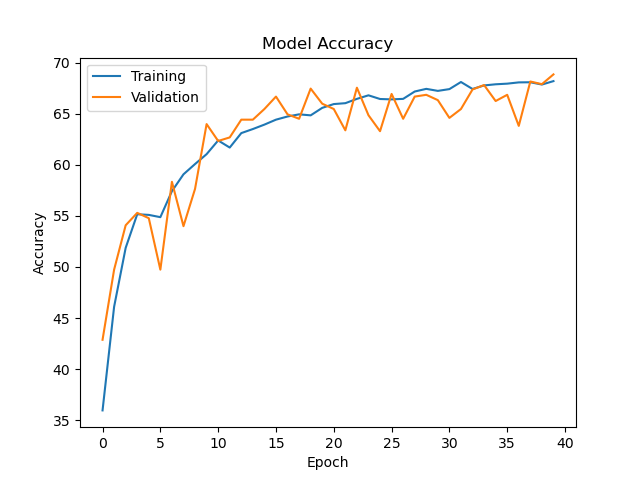
\includegraphics[width = 3in]{images/RNN_accuracies}
{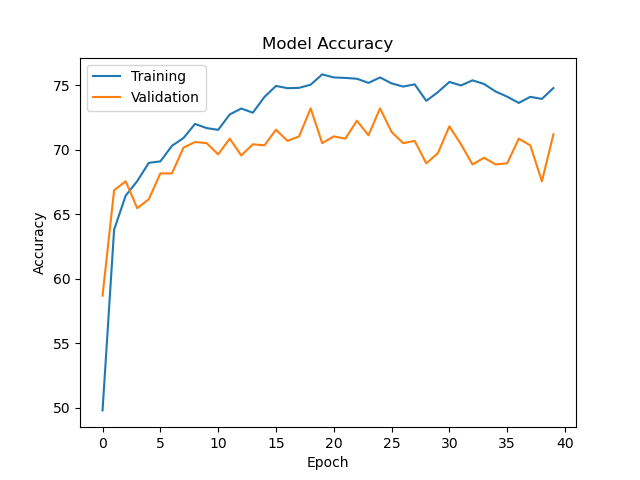
\includegraphics[width = 3in]{images/RNN_improved_accuracies}

\bigskip

Original Model Left, Improved Model Right

\bigskip

{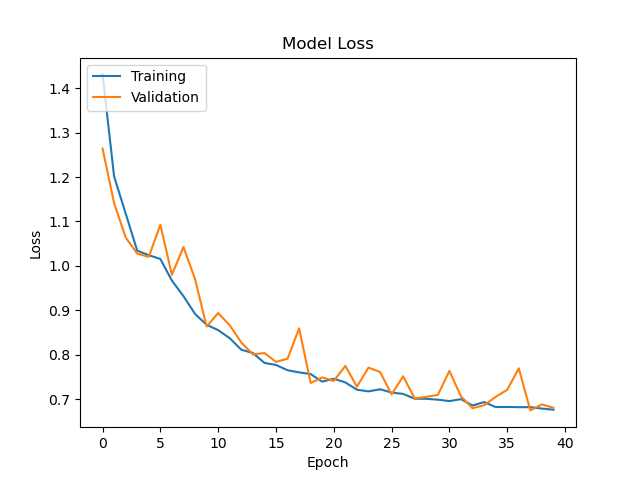
\includegraphics[width = 3in]{images/RNN_losses}
{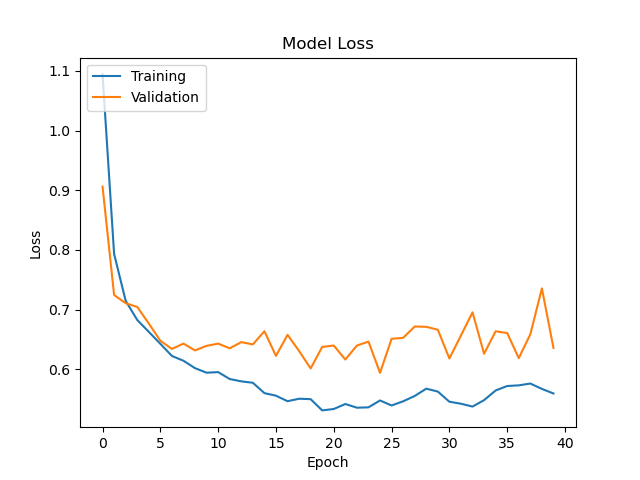
\includegraphics[width = 3in]{images/RNN_improved_losses}

\bigskip

Original Model Left, Improved Model Right

\bigskip

{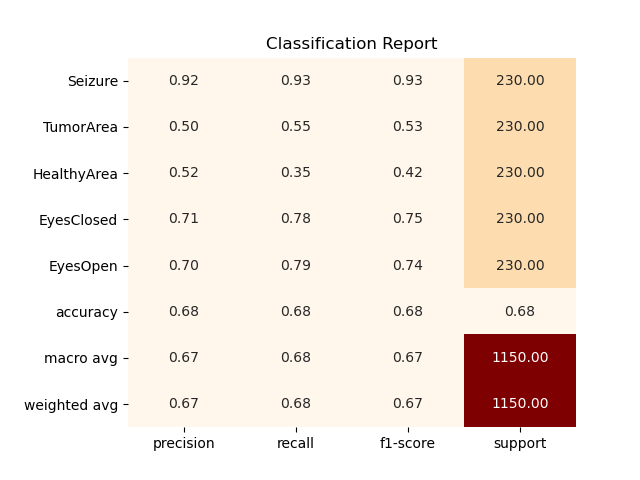
\includegraphics[width = 3in]{images/RNN_classification_report}
{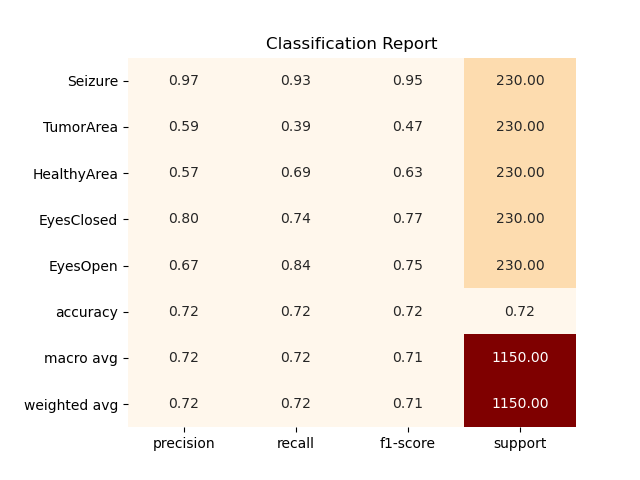
\includegraphics[width = 3in]{images/RNN_improved_classification_report}

\bigskip

Original Model Left, Improved Model Right

\bigskip

{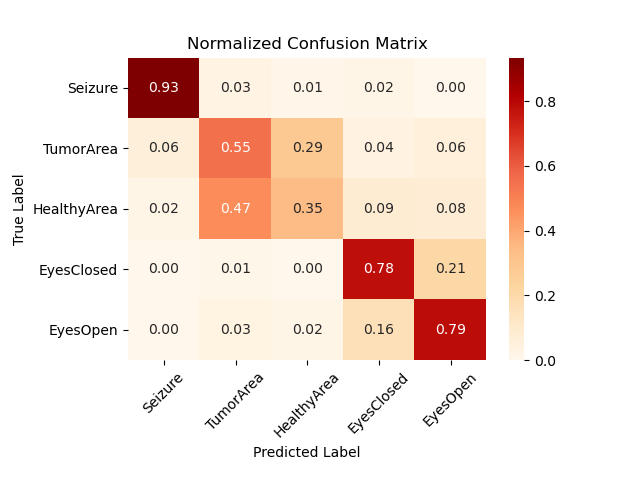
\includegraphics[width = 3in]{images/RNN_confusion_matrix}
{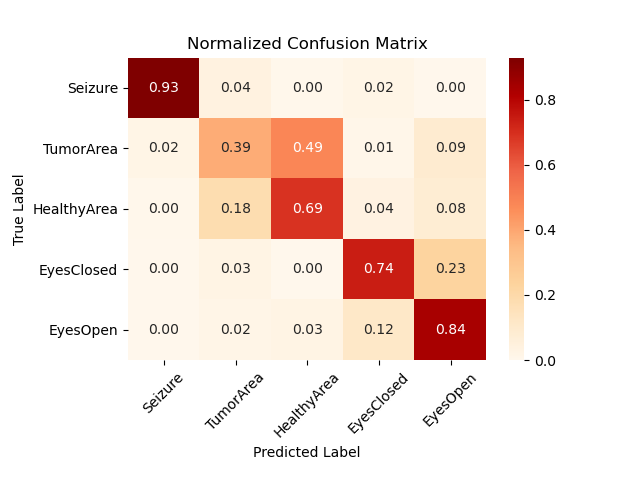
\includegraphics[width = 3in]{images/RNN_improved_confusion_matrix}

\textbf{d.} Explain your architecture and techniques used. Briefly discuss about the result with plots. [3 points]

\bigskip

My RNN improved model increased the hidden size of the GRU function to 256 values, added a 2nd hidden layer plus a dropout parameter value of 0.5. It also added 3 fully connected layers after thr GRU layer.  The 1st linear layer has 256 inputs and 128 outputs. The 2nd linear layer has 128 inputs and 64 outputs, and the output layer has 64 inputs and 5 outputs. 

\bigskip

My improved RNN model increased in ovrall accurcy from 0.68 to 0.72.  The loss dropped to below 0.70.  Most of the gains came from improvements in deecting Healthy Area, but it the false positives of healthy area that are truly tumor areas incresed as well.

\section{Mortality Prediction with RNN}

\subsection*{2.3 Building Model}

\bigskip

Original Model Left, Improved Model Right

\bigskip

{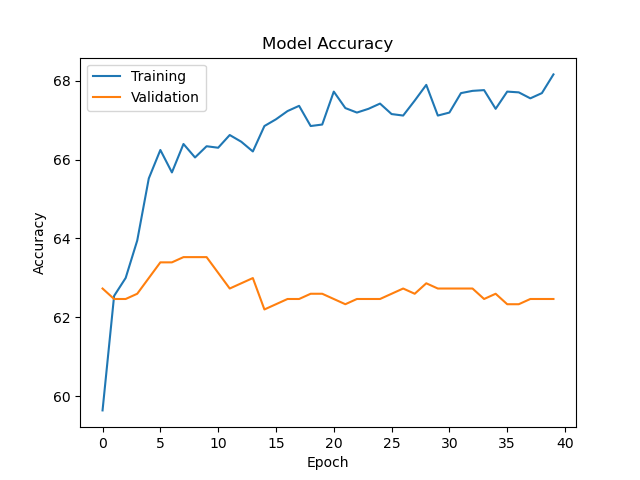
\includegraphics[width = 3in]{images/VAR_RNN_accuracies}
{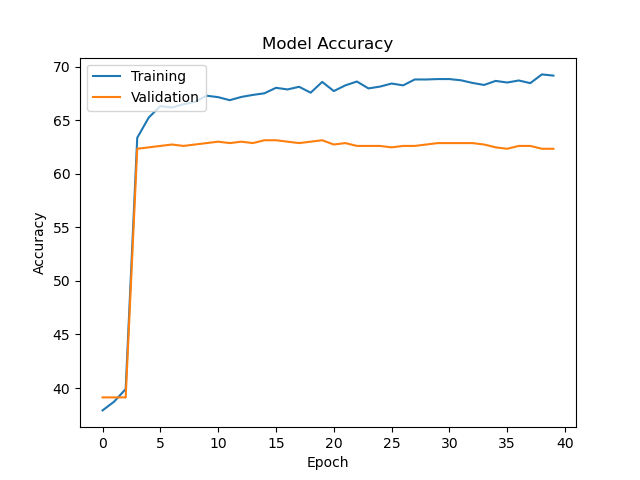
\includegraphics[width = 3in]{images/VAR_RNN_improved_accuracies}

\bigskip

Original Model Left, Improved Model Right

\bigskip

{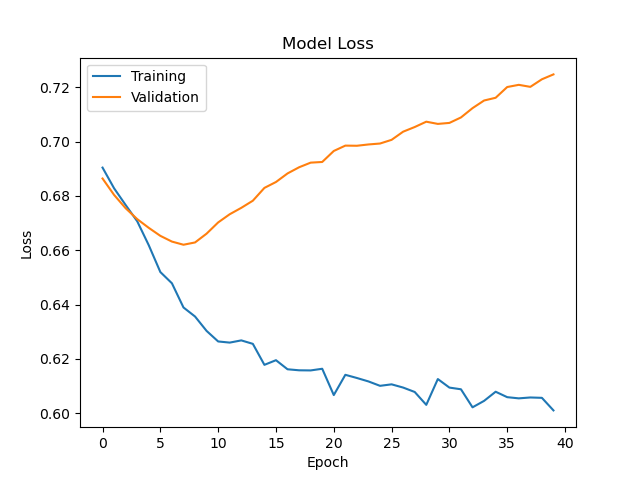
\includegraphics[width = 3in]{images/VAR_RNN_losses}
{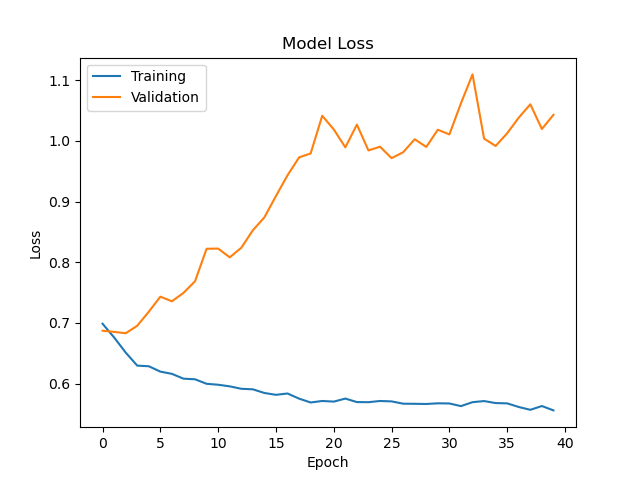
\includegraphics[width = 3in]{images/VAR_RNN_improved_losses}

\bigskip

Original Model Left, Improved Model Right

\bigskip

{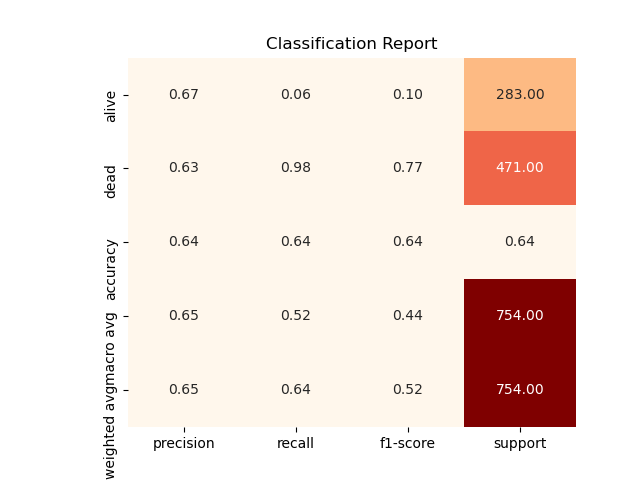
\includegraphics[width = 3in]{images/VAR_RNN_classification_report}
{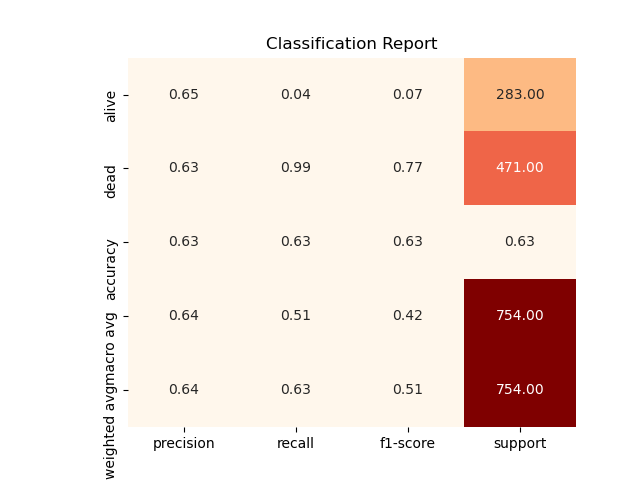
\includegraphics[width = 3in]{images/VAR_RNN_improved_classification_report}

\bigskip

Original Model Left, Improved Model Right

\bigskip

{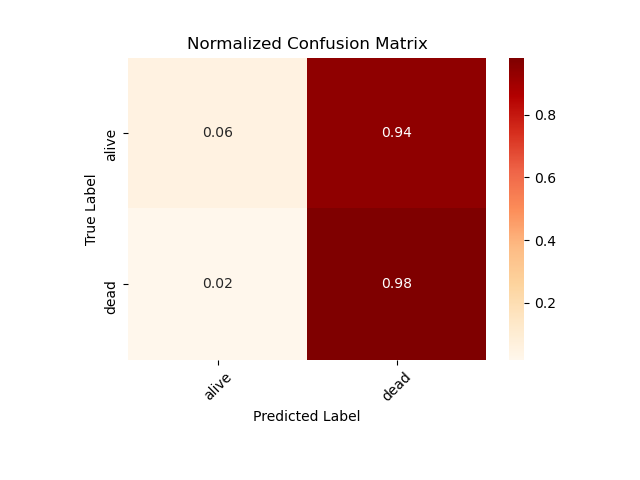
\includegraphics[width = 3in]{images/VAR_RNN_confusion_matrix}
{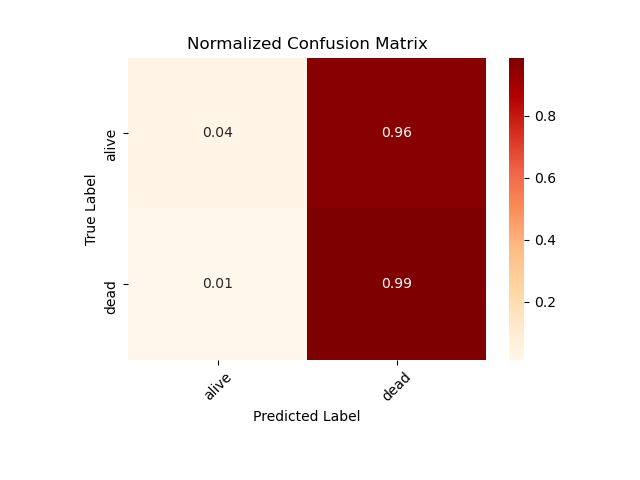
\includegraphics[width = 3in]{images/VAR_RNN_improved_confusion_matrix}

\bigskip

\textbf{b.} Explain your architecture and techniques used. Briefly discuss about the result with plots. [5 points]

\bigskip

My "improved" variable RNN model was modified over the original model by adding a fully connected layer prior to the GRU layer.  The GRU layer was modified by adding an extra hidden layer and a dropout parameter value of 0.50.  The 1st linear layer in front of the GRU layer consist of the custom input values and 128 features out. The 2nd linear layer is 128 inputs and 64 outputs.  The 2nd linear layer then passes through the tanh activation function prior to entering the GRU layer with 64 inputs and 16 outputs.  The output layer then has 16 inputs and 2 outputs.

\bigskip

My "improved" variable RNN model actually performs worse. The overall accuracy drops from 0.64 to 0.63.  The model is also overtrained to the training set.  The model loss also increase by approximately 0.30.

\end{document}
